\section{Visão geral da abordagem}
\label{sec:visão-geral}

Este trabalho adota uma abordagem empírica tendo como estudo de caso a migração da Self-Adaptive Body Sensor Network (SA-BSN) de ROS 1 Melodic, implementada em C++, para ROS 2 Jazzy, implementada em Python. O processo concentra-se na compreensão e sistematização do processo de migração, considerando as atividades realizadas, as decisões técnicas adotadas, os artefatos produzidos durante a evolução do sistema e os artefatos criados para refinar a sistematização posterior.

Assim, busca-se reconstruir o processo a partir das evidências disponíveis, identificando as atividades executadas e os critérios que fundamentaram as decisões de migração. A reconstrução considera os artefatos de desenvolvimento, incluindo código-fonte, especificações de requisitos, testes e histórico de implementação.

A sistematização do processo toma como referência uma abordagem orientada à preservação de comportamento no estabelecimento de um \textit{ground truth} comportamental do sistema legado e migração para ROS 2. A primeira fase começa com obtenção de conhecimento descrito sobre o sistema, a especificação dos comportamentos relevantes e o \textit{ground truth} comportamental. A segunda fase abrange a identificação das realizações desses comportamentos, a análise das transformações necessárias, a implementação no ambiente de destino e a validação dos comportamentos.

A Figura ~\ref{fig:metodologia} apresenta a
organização geral da abordagem e suas etapas.

\begin{figure}[htbp]
    \centering
    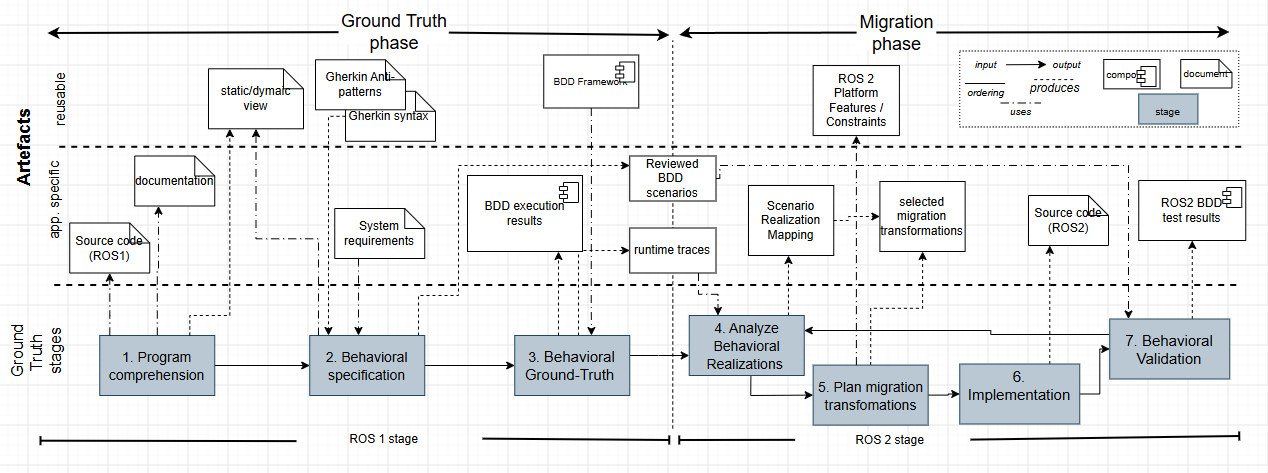
\includegraphics[width=1\textwidth]{img/metodologia.png}
    \caption{pipeline da metodologia}
    \label{fig:metodologia}
\end{figure}

Entretanto, a organização apresentada não pressupõe que todas essas atividades tenham sido executadas de maneira sistemática durante a migração original. Algumas etapas representam
práticas realizadas, enquanto outras correspondem a procedimentos refinados posteriormente para investigar ou complementar o processo. 


\section{Fase de \textit{Ground Truth} Comportamental}
\label{sec:fase-ground-truth}

A noção de recuperação de \textit{ground truth} adotada neste trabalho é inspirada no \textit{framework} proposto por Garcia et al.~\cite{GarciaKMD12}. Na abordagem desses autores, uma recuperação arquitetural autoritativa torna-se uma recuperação de \textit{ground truth} quando sua representação é examinada e certificada por um colaborador de longa data que possui conhecimento substancial da arquitetura do sistema.

A metodologia adapta o procedimento recuperação, avaliação e certificação por especialista para estabelecer uma \textit{Ground Truth} comportamental orientada por requisitos. Diferentemente de Garcia et al., cujo objetivo é recuperar elementos arquiteturais e suas relações com entidades de implementação, nosso objetivo é identificar os comportamentos esperados relevantes à migração e estabelecer como eles se manifestam no sistema legado.

O processo proposto adapta os papéis de (\textit{recoverer}) que coleta e interpreta evidências do sistema, formula especificações comportamentais e investiga sua execução na implementação legada e o (\textit{certifier}), que é um colaborador com conhecimento do domínio e da aplicação que revisa a interpretação dos requisitos e a \textit{Ground Truth} comportamental resultante. Essa revisão auxilia na identificação de ambiguidades, discrepâncias e conhecimentos específicos do sistema que não estejam adequadamente representados nos artefatos disponíveis.

Com base nesses princípios, a fase de \textit{Ground Truth} Comportamental é organizada nas etapas de Compreensão do Programa (\textit{Program Comprehension}), Especificação Comportamental (\textit{Behavioral Specification}) e \textit{Ground Truth} Comportamental (\textit{Behavioral Ground-Truth}).

A etapa de Compreensão do Programa fornece \textit{recoverer} conhecimentos estruturais, de execução e da aplicação da implementação legada. Esse conhecimento apoia a interpretação dos requisitos e a investigação do comportamento observável do sistema. Ele também permanece disponível para análises posteriores da implementação durante a fase de migração.

A etapa de Especificação Comportamental identifica, a partir das fontes disponíveis, os requisitos relevantes para a migração e expressa os critérios de aceitação selecionados como cenários BDD. O \textit{rec} utiliza os conhecimentos obtidos durante a Compreensão do Programa para interpretar os requisitos, enquanto o certificador, com conhecimento aprofundado do domínio e da aplicação, revisa os cenários BDD quanto à sua conformidade com o comportamento pretendido para o sistema. As especificações resultantes estabelecem as expectativas comportamentais a serem avaliadas.

Por fim, a etapa do \textit{Ground Truth} Comportamental implementa e executa os cenários no sistema legado. Os resultados observados são comparados aos critérios de aceitação especificados, e eventuais discrepâncias são investigadas. Essa atividade se apoia nos princípios de caracterização de sistemas legados discutidos por Feathers~\cite{Feathers2004}, que enfatizam a compreensão do comportamento existente antes de modificar a implementação.


\subsection{Compreensão de Programas}


A metodologia torna essa atividade preliminar de compreensão uma etapa explícita. Antes que as propriedades comportamentais possam ser identificadas para migração e que sua realização na implementação possa ser analisada, o \textit{recoverer} deve adquirir conhecimento suficiente sobre a organização e a execução do sistema legado. A Compreensão de Programas combina, portanto, conhecimento existente sobre o sistema com observações estruturais e de execução, apoiando a compreensão progressiva da implementação pelo \textit{Recoverer}.

Nesse sentido, é importante que um sistema possua ferramentas de documentação disponíveis que possam ajudar a formar esses modelos de conhecimento como o \textit{program model} e \textit{situation model} a partir de abordagens conhecidas como \textit{top-down}, como diagramas de arquitetura, diagramas de execução e ,para o nosso caso, artigos e abordagens \textit{bottom-up} que abrange código fonte, grafo de chamadas e grafo de dependência.

O objetivo desta etapa, é estabelecer o conhecimento contextual necessário para interpretar as evidências das etapas posteriores da migração. As informações estruturais ajudam a explicar como a implementação está organizada, enquanto as informações de execução revelam como os elementos do sistema se comunicam durante sua operação. Em conjunto com a documentação e o conhecimento do domínio, essas observações apoiam a especificação do comportamento legado e permanecem disponíveis para a interpretação posterior das entidades e dos componentes de implementação associados a esse comportamento.


\subsection{Especificação Comportamental}

A Especificação Comportamental propõe identificar os principais requisitos comportamentais para a migração e especificá-los na forma de contratos comportamentais representados por cenários BDD. Esses contratos estabelecem as condições de execução, os estímulos e os resultados observáveis esperados para os comportamentos selecionados.

Seguindo os papéis de \textit{recoverer} e \textit{certifier} adaptada de Garcia et al.~\cite{GarciaKMD12}, o \textit{recoverer} identifica e interpreta os requisitos comportamentais, enquanto o \textit{certifier} avalia se as especificações resultantes representam adequadamente o comportamento pretendido do sistema.

Os requisitos podem ter origem em propriedades formais, documentação do sistema, estudos anteriores mas é principalmente formulada pelo conhecimento da aplicação do próprio \textit{certifier} que descreve o comportamento geral do sistema. A Compreensão de Programas apoia a interpretação dessas fontes para o \textit{recoverer} que adapta o comportamento para linguagem \textit{Gerkhin} seguindo as boas práticas \cite{Binamungu}.

A metodologia proposta não prescreve um procedimento fixo para derivar cenários BDD a partir dos requisitos. Em vez disso, adota os princípios de especificação colaborativa do BDD, nos quais os comportamentos esperados são esclarecidos por meio de exemplos e da participação dos \textit{stakeholders}~\cite{Farooq2023BDD}. No nosso caso, o \textit{certifier} atua como \textit{stakeholder} que prioriza os comportamentos mais relevantes para migração além de diretamente informar esses requisitos. 

Diferentemente de uma especificação limitada à perspectiva de um usuário final, os cenários desta abordagem também podem descrever contratos comportamentais observáveis nas interfaces entre componentes, como a recepção de dados, a publicação de resultados ou o tratamento de indisponibilidade. O conhecimento técnico do \textit{certifier} pode auxiliar nessa delimitação sem desde que não haja uma imposição rígida em chamadas de métodos, classes ou decisões internas de arquitetura, que podem mudar durante a migração. A especificação registra o comportamento requerido e sua fronteira de observação, não uma implementação obrigatória.

A etapa produz cenários BDD revisado. Esse artefato fornece a expectativa comportamental necessária para o Estabelecimento do \textit{Ground truth} Comportamental, etapa na qual são executadas os testes para verificar se o comportamento prescrito condiz com a implementação do sistema. A figura \ref{fig:processobdd} demonstra esse procedimento.


\begin{figure}[H]
    \centering
    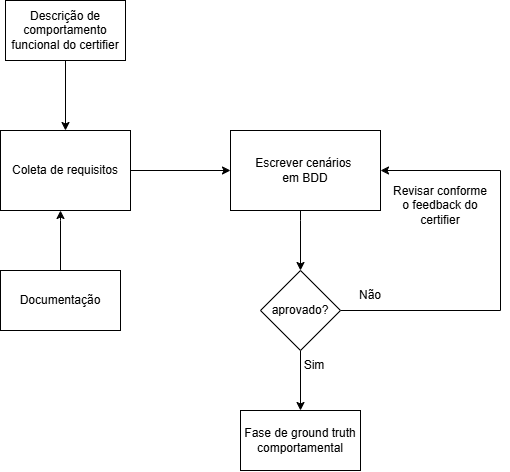
\includegraphics[width=0.7\textwidth]{img/especificacaoBDD.png}
    \caption{procedimento da especificação}
    \label{fig:processobdd}
\end{figure}




\subsection{Estabelecimento da \textit{Ground Truth} Comportamental}
\label{sec:ground-truth-comportamental}

A etapa de Especificação Comportamental estabelece os
comportamentos esperados do sistema a partir de requisitos
e critérios de aceitação expressos por meio de cenários BDD
e revisados com a participação do \textit{certifier}.
O Estabelecimento da \textit{Ground Truth} Comportamental
dá a continuidade do processo com objetivo de aplicar esses cenários
no sistema legado, relacionando os critérios de aceitação aos resultados observados por meio de testes. Essa organização tem precedência com a abordagem AAT4IRS, proposta por dos Santos et al. para testes de aceitação em sistemas robóticos \cite{Santos2024AAT4IRS} embora utilize garantias mais rígidas de teste.

Nesse sentido, os princípios dos testes de
caracterização permitem investigar e documentar
comportamentos existentes na implementação legada,
inclusive aqueles que não correspondem aos requisitos
especificados \cite{Feathers2004}.
Dessa forma, o comportamento esperado
estabelecido pelos critérios de aceitação e o
comportamento efetivamente observado durante a execução é uma lacuna relevante nessa etapa

O procedimento consiste em:

\begin{enumerate}

    \item \textbf{Preparar e executar os testes comportamentais:}

    Implementar as definições de \textit{steps} dos cenários BDD, incluindo as condições iniciais, os estímulos e as asserções necessárias para verificar os critérios de aceitação. A execução deve considerar as interfaces e os mecanismos disponíveis no ROS 1, podendo utilizar dados simulados, configurações de inicialização e registros de execução.

    Testes unitários, de integração e de caracterização podem complementar os cenários BDD na investigação de comportamentos específicos da implementação legada. Nesse trabalho foi feito a versão analisada, as condições de execução e os resultados dos testes.

    \item \textbf{Interpretar as evidências comportamentais:}

    Comparar os resultados observados com os critérios de aceitação, identificando os comportamentos que atendem aos requisitos, aqueles que apresentam discrepâncias e os casos em que as evidências são insuficientes para uma conclusão.

    As discrepâncias devem ser investigadas para distinguir possíveis defeitos da implementação, limitações dos testes e problemas de instrumentação. Quando necessário, testes adicionais podem complementar essa investigação. Quando a investigação identificar defeitos na implementação legada, é importante separar o comportamento originalmente observado daquele obtido após eventuais correções. Essas intervenções devem permanecer associadas às versões do código, aos critérios de aceitação e às evidências de correspondentes. Dessa forma, evita-se tratar uma implementação posteriormente corrigida como representação integral do comportamento histórico do sistema.


\end{enumerate}

Em paralelo ao estudo de Garcia Et al em que essa etapa requer uma participação rigorosa do \textit{certifier}, aqui ele pode ser consultado quando a interpretação das evidências suscitar
dúvidas sobre o comportamento pretendido,
mas não substitui a verificação baseada na
execução dos testes.

O estabelecimento do \textit{Ground Truth} comportamental permite verificar em que medida os cenários BDD correspondem a comportamentos
observáveis na implementação legada e se esses comportamentos satisfazem os critérios de aceitação definidos. Essa correspondência depende da adequação
dos testes, das condições de execução e das evidências obtidas.



\section{Fase de Migração}
\label{sec:fase-migracao}

A Fase de Migração utiliza a \textit{Ground Truth} comportamental estabelecida no ROS~1 para orientar a transformação da implementação legada e a preservação dos requisitos selecionados no ROS~2.

Essa fase adota a perspectiva \textit{white-box} e toma como referência o processo \textit{Horseshoe} discutido por Bragagnolo et al.~\cite{BragagnoloMigration}, que compreende o planejamento, a compreensão dos sistemas de origem e destino, a transformação do conhecimento adquirido e a produção do sistema de destino.

Na abordagem proposta, o planejamento geral delimita os requisitos e o escopo da migração. A Compreensão de Programas, a recuperação da \textit{Ground Truth} Comportamental e a Identificação das Realizações Comportamentais contribuem para a compreensão do sistema de origem. A compreensão do destino é incorporada ao Planejamento das Transformações de Migração, que examina as características do ROS~2 e utiliza o conhecimento recuperado para identificar as transformações necessárias. A Implementação corresponde à produção do sistema de destino.


A Validação Comportamental complementa o processo ao confrontar a referência estabelecida no ROS 1 com os comportamentos observados na implementação migrada, considerando os contratos comportamentais selecionados.


O que diferencia a nossa abordagem é a integração entre especificações BDD, evidências de implementação e transformações de migração além da atuação do \textit{recoverer} que analisa as evidências e reconstrói as transformações, enquanto o \textit{certifier} pode esclarecer restrições e expectativas comportamentais quando necessário, aprovar e revisar mudanças.




\section{Identificação das Realizações dos Comportamentos}
\label{sec:identificacao-realizacoes-comportamentos}

A identificação das realizações dos comportamentos busca relacionar os cenários BDD às entidades da implementação legada responsáveis por sua realização. A etapa parte da compreensão da implementação de origem, característica das abordagens \textit{white-box} de migração discutidas por Bragagnolo et al.~\cite{BragagnoloMigration}. A ideia é estabelecer relações rastreáveis entre os comportamentos especificados anteriormente, as entidades de implementação e suas respectivas responsabilidades, entendidas como atribuições funcionais ou operacionais desempenhadas por essas entidades, a fim de orientar a delimitação do escopo de investigação para o planejamento das transformações.

A análise do código legado como apoio à migração também é observada em Buchgeher et al.~\cite{BUCHGEHER2022276}, que utilizam análise estática para identificar variáveis, funções e instâncias relevantes à construção de modelos de informação para uma nova infraestrutura de comunicação. Nesta proposta, a investigação é orientada pelos requisitos e cenários BDD estabelecidos anteriormente, buscando identificar as entidades de implementação envolvidas na realização dos comportamentos selecionados.

Essa identificação é auxiliada por técnicas de
\textit{feature location}. Uma abordagem \textit{FeatureTrace}
\cite{BarbosaFeatureTrace} indica a possibilidade de estabelecer relações de rastreabilidade entre cenários BDD e métodos
exercitados durante a execução dos testes. Complementarmente, a técnica de \textit{Software Reconnaissance} \cite{WildeScully1995} fundamenta a análise comparativa da participação de elementos de código em diferentes funcionalidades. Em sistemas ROS, essas associações podem ser complementadas também pela \textit{RQT\_GRAPH} e documentações já disponíveis como as \textit{call graphs}.

O procedimento compreende quatro atividades:

\begin{enumerate}


    \item \textbf{Delimitar os comportamentos e suas interfaces:} A partir dos requisitos e cenários BDD estabelecidos na Especificação Comportamental, delimitar os contratos relevantes para a investigação de suas realizações, examinando suas condições iniciais, estímulos, resultados observáveis e implementações de teste. Identificar as interfaces ROS utilizadas para acionar ou observar esses comportamentos, incluindo tópicos, serviços, ações e parâmetros, e registrar as configurações de execução correspondentes.


    
    \item \textbf{Localizar as realizações na implementação legada:} Relacionar as interfaces identificadas ao grafo computacional ROS, aos arquivos de inicialização e ao código-fonte, identificando os nós e as entidades envolvidas na realização dos comportamentos. Quando disponíveis, utilizar evidências de execução e cobertura para complementar a localização de métodos e regiões de código candidatos, distinguindo a participação observada em execuções de testes das associações específicas entre cenários e entidades de implementação. Examinar as responsabilidades dos elementos identificados por meio da inspeção do código.


    \item \textbf{Caracterizar as responsabilidades
    e sua dependência de contexto:}
    examinar a participação dos elementos
    localizados nos comportamentos selecionados,
    identificando responsabilidades comuns,
    compartilhadas e específicas. Analisar suas
    dependências em relação ao ROS 1, diferenciando
    a lógica funcional relativamente independente
    da plataforma dos mecanismos de comunicação,
    execução, configuração, gerenciamento de
    estado e monitoramento vinculados ao contexto
    tecnológico. 

    \item \textbf{Consolidar o mapeamento e
    delimitar o escopo de transformação:}
    construir um \textit{Scenario Realization
    Mapping}, uma documentação que relacione os cenários BDD às
    entidades de código, aos componentes ROS,
    às interfaces de comunicação e às
    responsabilidades identificadas. A partir do mapeamento,
    selecionar as responsabilidades a serem
    aprofundadas no planejamento das
    transformações, justificando a seleção e
    registrando suas dependências de contexto.

\end{enumerate}

A etapa produz o \textit{Scenario Realization
Mapping}, um registro das responsabilidades
selecionadas para investigação no planejamento
da migração. 


\section{Planejamento das Transformações de Migração}
\label{sec:plan-migration-transformations}

O Planejamento das Transformações de Migração utiliza as responsabilidades delimitadas na etapa anterior para examinar como suas realizações devem ser tratadas diante da substituição do \textit{framework} ROS 1 pelo ROS 2. O procedimento sistematiza a relação entre o conhecimento recuperado da implementação legada e as características da plataforma de destino, em consonância com a compreensão do sistema de origem e o planejamento de mudanças discutidos por Bragagnolo et al.~\cite{BragagnoloMigration}.


A análise considera os princípios associados ao \textit{system context} discutidos por Garcia et al.~\cite{GarciaKMD12}, examinando como serviços de comunicação, gerenciamento de nós, configuração e execução influenciam a realização das responsabilidades identificadas. A relevância
dessas dependências também é observada em Buchgeher et al.~\cite{BUCHGEHER2022276}, que
descrevem a migração de uma infraestrutura proprietária de comunicação para OPC UA, preservando grande parte da camada de controle e adaptando os componentes necessários à sua integração com a nova arquitetura. Nesta etapa, busca-se examinar quais responsabilidades
podem manter sua lógica funcional e quais mecanismos precisam ser adaptados, reorganizados
ou ampliados diante das características do ROS 2.

Nesse contexto, é possível avaliar três perspectivas de transformação, a adaptação do \textit{System context} relacionado a mudança de framework, a refatoração interna motivada por melhorias de qualidade como modularidade e testabilidade. E evolução funcional que amplia a capacidade do sistema. Na BSN, por exemplo, a reorganização do processamento e da classificação de risco pode ser analisada como refatoração interna, enquanto a adoção de nós com ciclo de vida gerenciado envolve diretamente recursos do ROS 2. A ampliação do monitoramento por eventos e \textit{heartbeats}, por sua vez, deve ser examinada como uma evolução das responsabilidades de observação, e não como consequência obrigatória da plataforma.

O procedimento consiste em:

\begin{enumerate}

    \item \textbf{Examinar as diferenças entre os
    contextos de implementação:}

    Comparar os mecanismos utilizados no ROS~1
    com os recursos e modelos de execução
    disponíveis no ROS~2, considerando as
    responsabilidades delimitadas na etapa
    anterior.

    A análise busca distinguir adaptações
    necessárias à substituição do
    \textit{framework} de possibilidades
    de reorganização ou ampliação das
    responsabilidades existentes.

    \item \textbf{Identificar e caracterizar
    as transformações de migração:}

    Relacionar as entidades da implementação
    legada às estruturas correspondentes
    no ROS~2, identificando as transformações
    realizadas ou previstas.

    As transformações podem envolver adaptação
    à plataforma, preservação da lógica
    funcional, reorganização interna ou
    evolução de comportamento, sendo essas
    classificações não mutuamente exclusivas.

    No estudo retrospectivo, a caracterização
    considera o código-fonte e a documentação
    disponível, distinguindo as motivações
    documentadas das interpretações
    decorrentes da análise.

    \item \textbf{Relacionar as transformações
    aos contratos comportamentais e
    consolidar o registro:}

    Utilizar o \textit{Scenario Realization
    Mapping} para identificar os contratos
    associados às responsabilidades
    transformadas e examinar possíveis
    repercussões sobre seus comportamentos
    observáveis.

    A análise distingue contratos cuja
    preservação deve ser verificada de
    comportamentos adicionais introduzidos
    durante a migração.

    As associações são consolidadas em um
    \textit{Migration Transformation Record},
    relacionando as responsabilidades de
    origem, as realizações no ROS~2,
    o tratamento identificado e os
    contratos comportamentais pertinentes.

\end{enumerate}


A caracterização das transformações pode ser complementada pela análise de métricas estruturais das entidades envolvidas. Medidas de complexidade ciclomática, complexidade das classes, coesão e acoplamento permitem examinar características da organização interna da implementação e complementar a interpretação das responsabilidades identificadas \cite{McCabe1976,ChidamberKemerer1994}. A análise deve considerar a correspondência entre as entidades examinadas e as definições operacionais das métricas utilizadas, especialmente quando a migração envolve mudanças de linguagem e de decomposição dos componentes. Essas medidas são utilizadas como evidências complementares para caracterizar as transformações, sem pressupor que diferenças numéricas demonstrem, isoladamente, melhorias de qualidade estrutural.



O resultado da etapa é o \textit{Migration Transformation Record}, que sintetiza as correspondências entre responsabilidades da implementação legada, transformações previstas ou identificadas na implementação de destino e contratos comportamentais associados. As evidências e justificativas são complementadas pela análise de cada transformação. No estudo retrospectivo, esse registro permite caracterizar as mudanças observadas nas implementações, sem pressupor que tenham sido planejadas conforme a abordagem proposta.


\subsection{Implementação}

A Implementação concretiza as transformações
definidas na etapa de Planejamento das
Transformações de Migração, produzindo a
implementação do sistema no ambiente de destino.

Seguindo a perspectiva \textit{white-box}
discutida por Bragagnolo et al.~
\cite{BragagnoloMigration}, a implementação
migrada pode diferir do sistema legado em
linguagem de programação, organização de
componentes, interfaces, dependências e
mecanismos específicos da plataforma.

As atividades de implementação compreendem
a adaptação ou substituição dos mecanismos
dependentes da plataforma de origem, bem como
a reorganização das responsabilidades dos
componentes quando necessária. Dependendo
das transformações selecionadas, partes do
sistema podem ser reutilizadas, modificadas
ou reescritas para atender às características
do ambiente de destino.

Testes unitários, de componentes e de
integração podem apoiar a identificação de
defeitos durante o desenvolvimento. Contudo,
a investigação sistemática da preservação
dos comportamentos selecionados pertence
à etapa posterior de Validação Comportamental.

A etapa visa produzir a implementação do sistema
migrado, composta pelo código-fonte,
configurações, interfaces e demais artefatos
necessários à sua execução na plataforma
de destino.

\subsection{Validação Comportamental}
\label{sec:validacao-comportamental}

A Validação Comportamental investiga em que medida a implementação migrada satisfaz os principais requisitos comportamentais e preserva os contratos considerados relevantes da implementação legada por meio da execução de testes em BDD. Nesse contexto, alguns estudos indicam essa relação de validação por teste como em  Khodabandehloo et al.~\cite{Khodabandehloo2021} que apresentam uma abordagem de testes aplicada à reengenharia de sistemas legados, na qual testes automatizados apoiam a verificação das funcionalidades durante a transformação do sistema.

A etapa utiliza os requisitos e cenários BDD
da Especificação Comportamental, 
com a referência e as ressalvas identificadas
no Estabelecimento da \textit{Ground Truth}
Comportamental para verificar a conformidade. 

O procedimento consiste em:

\begin{enumerate}

\item \textbf{Estabelecer correspondências
comportamentais:}
Identificar cenários e critérios de aceitação
relacionados nas duas implementações,
considerando seu significado e não apenas
a identidade de nomes ou arquivos.
Essa atividade considera o princípio de
comparação entre observações correspondentes
de diferentes versões, explorado por
Insa et al.~\cite{Insa2018}.
Identificar os cenários reutilizados,
adaptados, introduzidos ou sem contraparte,
considerando as versões investigadas.

\item \textbf{Adaptar os testes e examinar
a instrumentação:}

Implementar testes comportamentais
para sua execução no ambiente de destino,
preservando os critérios de aceitação relevantes
dos cenários BDD.

Essa atividade propõe adaptar as
definições de passos, das condições iniciais,
dos estímulos, dos mecanismos de observação,
das asserções e da infraestrutura de inicialização
e execução dos testes para o ambiente do ROS 2 e examinar a correspondência entre as duas implementações, considerando diferenças de interfaces, configurações, mecanismos de inicialização e janelas de observação.

\item \textbf{Interpretar discrepâncias
e consolidar os resultados:}
Investigar candidatos a regressão, correções intencionais, mudanças de contrato, falhas de instrumentação e resultados inconclusivos. Considerar a produção efetiva dos estímulos, a validade das asserções e a compatibilidade das condições de execução antes de atribuir uma divergência à migração.

\end{enumerate}

A aprovação de testes nas duas implementações
não demonstra, por si só, equivalência
comportamental. As conclusões dependem da
correspondência entre os critérios de aceitação,
estímulos, observações e versões investigadas.

A etapa produz uma suíte de testes comportamentais adaptada à implementação migrada, incluindo as definições de passos, as asserções e a infraestrutura necessária à execução dos cenários BDD selecionados. Sua aplicação fornece evidências sobre a satisfação dos requisitos e a preservação de contratos comportamentais, acompanhadas das discrepâncias e limitações da comparação. Em estudos retrospectivos, a suíte e suas evidências podem ser recuperadas a partir dos artefatos existentes.



